Today, Don suggested working on ice core data drilled from Antartica, Vostok. The data contains history of temperature, \ce{CO2}, \ce{CH4}, and other proxies for over 420,000 years ~\citep{PJR-JJ-RD:1999}.
\begin{enumerate}
  \item The complete data set is avaiable at \path{ftp://ftp.ncdc.noaa.gov/pub/data/paleo/icecore/antarctica/vostok/}
  \item Under the guidance of Don, we generated several plots:
    \begin{enumerate}
      \item 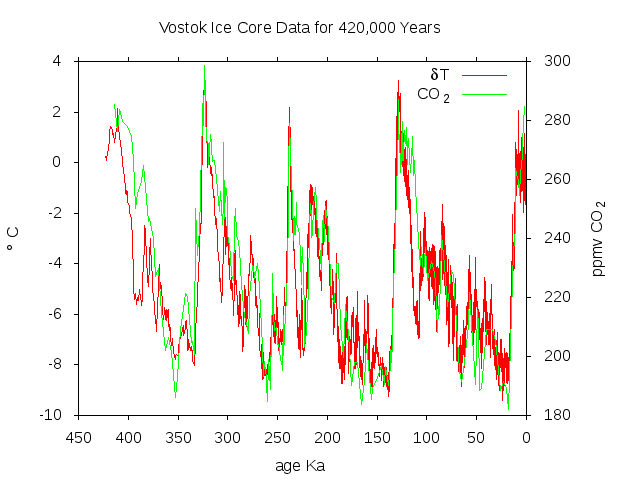
\includegraphics[scale=0.5]{00LOG/2017-07-12/00FIGURES/VOSTOK_T_CO2.png}
      \item 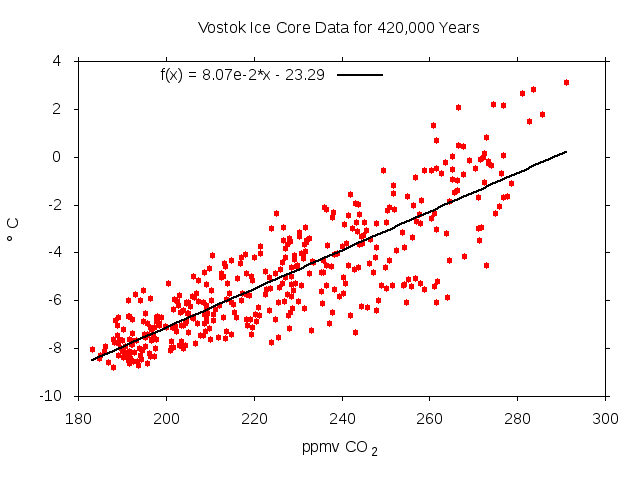
\includegraphics[scale=0.5]{00LOG/2017-07-12/00FIGURES/VOSTOK_ppmv_CO2_vs_deltaT_linear_fit.png}
      \item 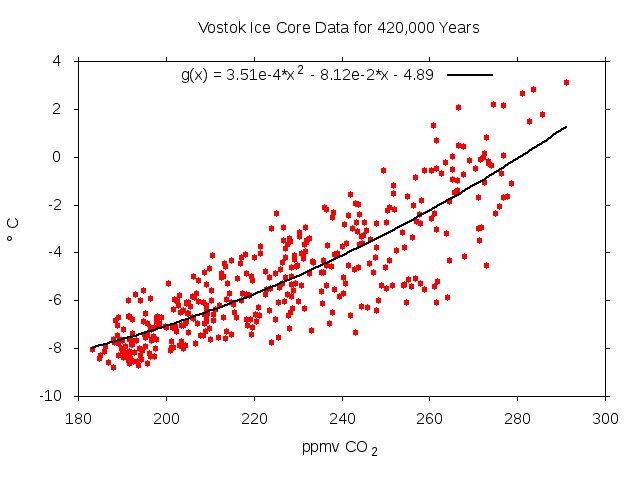
\includegraphics[scale=0.5]{00LOG/2017-07-12/00FIGURES/VOSTOK_ppmv_CO2_vs_deltaT_quadratic_fit.png}
    \end{enumerate}
\end{enumerate}
